
\documentclass[11pt,addpoints,letterpaper]{exam}
\usepackage{adjustbox} % Add this to the preamble
\usepackage{float}

\usepackage{amsmath,tcolorbox,mdframed,xcolor}
\usepackage[top=0.75in, bottom=0.85in, left=1in, right=1in]{geometry} % Adjust margins
\usepackage{mathtools}
\usepackage{siunitx}
\usepackage{nccmath}
\usepackage{physics}
\usepackage{tikz}
\usepackage{multicol}
\usepackage{epigraph}
\usepackage{cancel}
\usepackage{xfrac}
\usepackage{pgfplots}
\usepackage{array}   % For alignment
\usepackage{booktabs} % For better horizontal lines
\usepackage{caption} % For caption formatting
\usepackage{graphicx} % For scaling tables if needed
\usepackage{setspace}

\setlength\epigraphwidth{.8\textwidth}
\setlength\epigraphrule{0pt}

\noprintanswers

\newcommand{\Section}[1]{
\textbf{\\\Large #1\\}
}
\newcommand{\labheader}[4]{%
  \vspace*{-0.2in} % Adjust vertical spacing
  \noindent
  \makebox[0.65\textwidth][l]{Name:\enspace\hrulefill\,\,\,}
  \makebox[0.1\textwidth][l]{\,Period:\enspace}
  \makebox[0.25\textwidth][l]{\hrulefill}\\[0.25cm]
  \makebox[0.65\textwidth][l]{Instructor: \enspace\texttt{\underline{#1}}}\hfill
  \makebox[0.1\textwidth][l]{ Course: }\hfill 
  \makebox[0.25\textwidth][l]{ \texttt{\underline{#2}}}\hfill \\[0.25cm]
  \makebox[0.65\textwidth]{}\makebox[0.1\textwidth][l]{ Term: }\hfill
  \makebox[0.25\textwidth][l]{\enspace\texttt{\underline{#3}}}\hfill
  % \hfill{Score: \underline{\hspace{2cm}}/#4}
  \vspace{0.5in}
}

% Define variables
\newcommand{\instructor}{Mr. Rodriguez}
\newcommand{\coursename}{Conceptual Physics A}
\newcommand{\term}{Winter}
\newcommand{\courseyear}{2024-2025} % Renamed \year to \courseyear to avoid conflict
\newcommand{\instructions}{}
\newcommand{\worksheetname}{Lab 4: Inertia and Oscillations}
\newcommand{\qspppp}{\vspace{6cm}}
\newcommand{\qsppp}{\vspace{4.5cm}}
\newcommand{\qspp}{\vspace{2.5cm}}
\newcommand{\qsp}{\vspace{0.6cm}}

\tcbset{
    myboxstyle/.style={
        colback=white,        % Background color
        colframe=black,       % Border color
        boxrule=0.5pt,        % Border thickness
        arc=5mm,              % Rounding radius
        boxsep=2mm,           % Padding around text
        left=4pt, right=4pt,  % Inner padding on left and right
    }
}
\newcommand{\equationbox}[2]{
\begin{center}
\begin{tcolorbox}[colframe=black!60, colback=white, arc=5mm, boxrule=0.75pt, title=#1]
% \vspace{-0.2in} % Tightens the space between the title and content
\begin{flushleft}
\begin{align}
#2
\end{align}
\end{flushleft}
\end{tcolorbox}
\end{center}
}
\newcommand{\equationboxx}[2]{
\begin{center}
\begin{tcolorbox}[colframe=black!60, colback=white, arc=5mm, boxrule=0.75pt, title=#1]

#2

\end{tcolorbox}
\end{center}
}
\newcommand{\instructionbox}[1]{\begin{center}\fbox{\fbox{{\centering #1}}}\end{center}}

\newcommand{\learningStandard}[1]{
    \small
    \tcbox[colback=gray!10, colframe=black, boxrule=0.5mm, sharp corners=southwest]{
        \textbf{#1} \hspace{0.5cm} % Spacing between title and vertical rule
        \textcolor{gray}{\vrule height 10pt width 0.3pt}\hspace{0.5cm} % Lighter and thinner vertical rule
        \textbf{Score:} \rule{1.5cm}{0.5pt} /10
    }
}

\newtcolorbox{learningStandardBox}[2]{%
    title={Learning Standard #1}, % Title with manual input for the standard number
    fonttitle=\bfseries\small,  % Title font style
    colback=gray!15, % Background color for main content
    colframe=black, % Frame color
    coltitle=black!80, % Font color for title
    colbacktitle=gray!60, % Background color for title
    boxrule=0.5mm, % Border thickness
    sharp corners=south, % Rounded top corners only
    width=\textwidth, % Full text width
    halign=center, % Center-align content
    top=10pt, % Adds extra space at the top to move content down
}
\newcommand{\standardBox}[2]{%
    \begin{learningStandardBox}{#1}{#2} % Passes number and name as arguments
        \begin{minipage}[t]{0.5\textwidth} % Left section for standard name
            \textit{#2} % Italicized name of the standard
        \end{minipage}%
        \hfill
        \begin{minipage}[t]{0.25\textwidth} % Middle section for score
            \textbf{Score:} \rule{1.5cm}{0.5pt} /10
        \end{minipage}%
        \hfill
        \begin{minipage}[t]{0.2\textwidth} % Right section for grade
            \textbf{Grade:} \phantom{1.2cm}
        \end{minipage}
    \end{learningStandardBox}
}
\newcommand{\standardBoxnoscore}[2]{%
    \begin{learningStandardBox}{#1}{#2} % Passes number and name as arguments
        \begin{minipage}[t]{0.5\textwidth} % Left section for standard name
            \textit{#2} % Italicized name of the standard
        \end{minipage}%
        \hfill
        \begin{minipage}[t]{0.25\textwidth} % Middle section for score
            \textbf{Score:} \rule{1.5cm}{0.5pt} /0
        \end{minipage}%
        \hfill
        \begin{minipage}[t]{0.2\textwidth} % Right section for grade
            \textbf{Grade: N/A} \phantom{1.2cm}
        \end{minipage}
    \end{learningStandardBox}
}


\newcommand{\exampleBox}[2]{%
    \begin{tcolorbox}[title=\texttt{Example}]
        \texttt{Problem:} {#1\\} 
        \texttt{Solution:} {#2}
    \end{tcolorbox}%
}

\newcommand{\customsection}[1]{%
    \vspace{1em} % Add some vertical space above (optional)
    {\Large\bfseries #1} % Format the title: large font and bold
    \par\vspace{0.5em}\noindent % Add some space below
}

\addpoints
\noprintanswers

\begin{document}

\labheader{Mr. Rodriguez}{Conceptual Physics A}{Winter 2024-25}{\numpoints}

\begin{centering}
\noindent\textbf{\\\Large Midterm Exam v2\\} 
\end{centering}

\qsp
\instructionbox{Be sure to show your work, include units when appropriate, and box your answers.}
\qsp

\standardBox{1}{Scientific Measurement and Estimation}

\begin{table}[h!]
\centering

\begin{tabular}{l c c c l}
\toprule
\textbf{Prefix} & \textbf{Symbol} & \textbf{Meaning} & \textbf{Expanded Form} & \textbf{Scientific Form}\\
\midrule
giga- & G & one billion & 1,000,000,000 & $\hspace{4ex}\times 10^{9}$\\ 
mega- & M & one million & 1,000,000 & $\hspace{4ex}\times 10^{6}$\\ 
kilo- & k & one thousand & 1,000 & $\hspace{4ex}\times 10^{3}$\\ 
hecto- & h & one hundred & 100 & $\hspace{4ex}\times 10^{2}$\\ 
-- & -- & one & 1 & $\hspace{4ex}\times 10^{0}$\\ 
centi- & c & one hundredth & 0.01 & $\hspace{4ex}\times 10^{-2}$\\ 
milli- & m & one thousandth & 0.001 & $\hspace{4ex}\times 10^{-3}$\\ 
micro- & $\mu$ & one millionth & 0.000001 & $\hspace{4ex}\times 10^{-6}$\\ 
nano- & n & one billionth & 0.000000001 & $\hspace{4ex}\times 10^{-9}$\\ 
\bottomrule
\end{tabular}
\captionsetup{font=small, labelfont=bf}
\caption{Metric Prefixes Conversion Chart}
\end{table}

\begin{questions}


\question[2] Place either a $<$, $>$, or $=$ sign in the blank.

\begin{parts}
    \part \SI{2500}{mL} \underline{\hspace{1cm}} \SI{2.5}{L}
    \part \SI{0.8}{km} \underline{\hspace{1cm}} \SI{800}{m}
    \part \SI{150}{g} \underline{\hspace{1cm}} \SI{0.15}{kg}
    \part \SI{0.000001}{m} \underline{\hspace{1cm}} \SI{1}{\mu m}
\end{parts}

\qsp

\question[2] Fill in the blank with the correct number.

\begin{parts}
    \part \SI{8}{kg} = \underline{\hspace{2cm}} g
    \part \SI{920}{g} = \underline{\hspace{2cm}} kg
    \part \SI{0.45}{km} = \underline{\hspace{2cm}} m
    \part \SI{5000}{m} = \underline{\hspace{2cm}} cm
\end{parts}

\qsp 

\question[2] Express each of the following in scientific notation:

\begin{parts}
    \part 0.000089 = \underline{\hspace{5cm}}
    \part 7340000 = \underline{\hspace{5cm}}
\end{parts}

\qsp

\question[2] Express each of the following in decimal (expanded) form:

\begin{parts}
    \part $3.142 \times 10^{8}$ = \underline{\hspace{5cm}}
    \part $6.2 \times 10^{-5}$ = \underline{\hspace{5cm}}
\end{parts}
\qsp
\question[2] In your own words, provide at least \textbf{two} reasons as to why the metric system is useful to scientists.  

\qspp

\newpage
\standardBox{2}{Linear Motion}

\equationboxx{Relevant Equations}{
\begin{align*}
x &= \frac{1}{2} a t^2 & & \text{(position equation)}\\
v &= at & & \text{(velocity equation)}
\end{align*}
}

\question[3] Sonic the Hedgehog is running a marathon. Once he starts running, he is capable of accelerating at $\SI{1.75}{m/s^2}$ indefinitely. If he runs for 27 minutes, how \textbf{far} will he travel? (\emph{Hint:} Convert minutes to seconds)

\qspppp

\question[3] Mr. Rodriguez is driving a 2007 Lincoln Town Car. To merge onto the freeway, he needs to accelerate at $a=\SI{2.5}{m/s^2}$. If he keeps accelerating at this same rate for $t=\SI{11}{s}$ how \textbf{fast} will he be going once he takes his foot off of the gas pedal?

\qspppp
\newpage
\begin{spacing}{1.5}
\question[1] \textbf{Acceleration} ($a$) is defined as a change in \underline{\hspace{5cm}} divided by a change in \underline{\hspace{5cm}}. \qsp


\question[1] \textbf{Displacement} ($\Delta x$) is defined as a change in \underline{\hspace{5cm}} and has units of \underline{\hspace{5cm}}. 

\end{spacing}


\qsp


\question[2] For each of the ticker-tape data below, \textbf{draw a corresponding curve} on a position vs. time graph that captures the motion qualitatively:
\begin{parts}

\begin{figure}[H]
    \centering
        \caption{Ticker-Tape Trial \textbf{A}}

    % \vspace{0.2cm} % Add vertical space above the image
  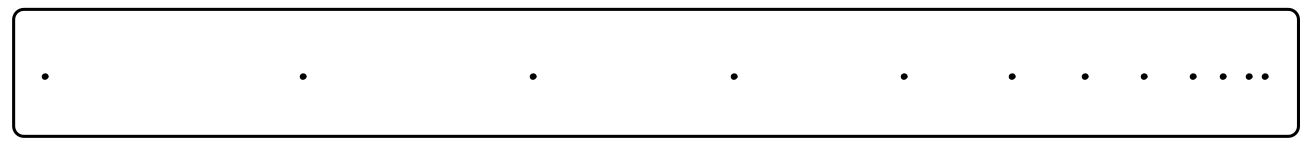
\includegraphics[width=0.9\textwidth]{a.png} % Specify image width and file name
\end{figure}

\qsp

\part Draw the curve corresponding to Ticker-Tape Trial \textbf{A} in the space provided below:

\qsp 

\begin{centering}
\begin{tikzpicture}[>=stealth, semithick]
    % x-axis
    \draw[->] (0,0) -- (10,0) 
        node[anchor=north east]{Time};

    % y-axis with vertically centered label
    \draw[->] (0,0) -- (0,6)
        % Place label halfway up, rotate by 90°, and shift left a bit
        node[midway, rotate=90, yshift=1em]{Position};
\end{tikzpicture}
\end{centering}

\qsp

\newpage

\begin{figure}[H]
    \centering
        \caption{Ticker-Tape Trial \textbf{B}}

    % \vspace{0.2cm} % Add vertical space above the image
  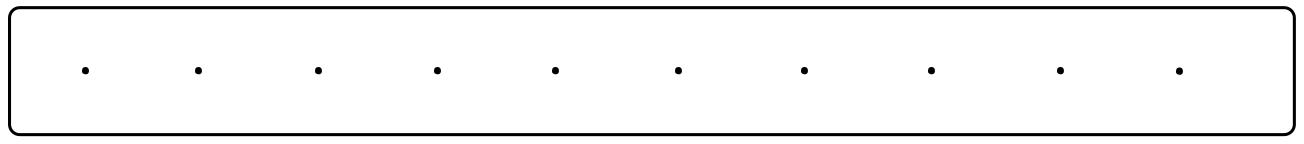
\includegraphics[width=0.9\textwidth]{b.png} % Specify image width and file name
\end{figure}


\part Draw the curve corresponding to Ticker-Tape Trial \textbf{B} in the space provided below:

\qsp 

\begin{centering}
\begin{tikzpicture}[>=stealth, semithick]
    % x-axis
    \draw[->] (0,0) -- (10,0) 
        node[anchor=north east]{Time};

    % y-axis with vertically centered label
    \draw[->] (0,0) -- (0,6)
        % Place label halfway up, rotate by 90°, and shift left a bit
        node[midway, rotate=90, yshift=1em]{Position};
\end{tikzpicture}
\end{centering}

\qsp

\begin{figure}[H]
    \centering
        \caption{Ticker-Tape Trial \textbf{C}}

    % \vspace{0.2cm} % Add vertical space above the image
  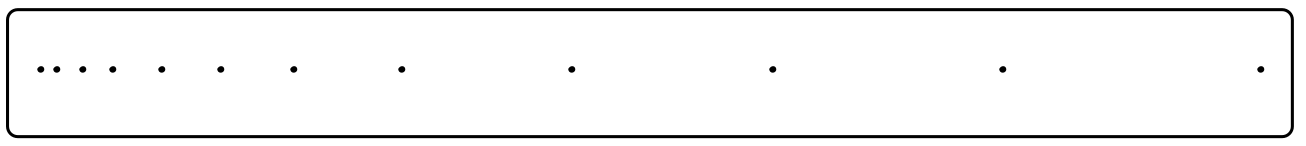
\includegraphics[width=0.9\textwidth]{c.png} % Specify image width and file name
\end{figure}


\part Draw the curve corresponding to Ticker-Tape Trial \textbf{C} in the space provided below:

\qsp 

\begin{centering}
\begin{tikzpicture}[>=stealth, semithick]
    % x-axis
    \draw[->] (0,0) -- (10,0) 
        node[anchor=north east]{Time};

    % y-axis with vertically centered label
    \draw[->] (0,0) -- (0,6)
        % Place label halfway up, rotate by 90°, and shift left a bit
        node[midway, rotate=90, yshift=1em]{Position};
\end{tikzpicture}
\end{centering}

\qsp

\end{parts}

\newpage
\standardBox{3}{Newton's Laws and Forces}

\equationboxx{Relevant Equations}{
\begin{align*}
\vb{F} &= m\vb{a}
\end{align*}
}

\question[1] What is Newton's \textbf{First} Law? 

\begin{choices}
\choice For every action, there is an equal and opposite reaction. 
\choice An object will only change its state of motion or rest if acted upon by an external force.
\choice All objects move in straight lines forever.
\choice The force exerted on an object is equal to its mass times its acceleration.
\end{choices}

\qsp

\question[1] What is Newton's \textbf{Second} Law? 

\begin{choices}
\choice All objects move in straight lines forever.
\choice An object will only change its state of motion or rest if acted upon by an external force.
\choice The net force exerted on an object is equal to its mass times its acceleration.
\choice For every action, there is an equal and opposite reaction.
\end{choices}

\qsp

\question[1] What is Newton's \textbf{Third} Law? 

\begin{choices}
\choice The force exerted on an object is equal to its mass times its acceleration.
\choice An object will only change its state of motion or rest if acted upon by an external force.
\choice All objects move in straight lines forever.
\choice For every action, there is an equal and opposite reaction.
\end{choices}

\qsp

\question[2] 
\qsp
\begin{parts}
\part Is your \textbf{mass} the same on the planet \textbf{Mars} as it would be on the planet $\textbf{Venus}$? 

\qspp

\part What about your \textbf{weight}? Why or why not?

\qspp

\end{parts}

\question[3] You are on a spaceship deep in outer space, far away from any planets or stars (\textit{i.e.}, there is \textbf{no gravity}). In your large and otherwise empty spaceship, there are two unmarked, equally sized boxes floating next to you. One box is full of feathers, and the other is full of solid lead. Explain in \textbf{2-3 complete sentences} how you can perform a simple experiment while exploiting Newton's Second Law to determine which box is full of feathers and which box is full of lead. (You cannot look inside the boxes.) 

\qspppp
\qsp


\question[2] You are on planet Earth. In a gleeful mood, you decide to jump up into the air. 
\begin{parts}
\part While you are in the air, how do the gravitational \textbf{forces} between you and planet Earth compare?

\qsppp

\part While you are in the air, how do the magnitudes of the \textbf{accelerations} of you and planet Earth compare?

\end{parts}

\qspppp



\qsp

\newpage
\standardBox{4}{Momentum}
\equationboxx{Relevant Equations}{
\begin{align*}
\vb{p} &= m\vb{v}
\end{align*}
}

\question[1] Choose \textbf{\emph{one}}: In which of the following scenarios is \textbf{momentum} conserved?
\begin{choices}
\choice An elastic collision.
\choice A partially inelastic collision
\choice A perfectly inelastic collision. 
\choice Momentum is conserved in all collisions, assuming no external forces.
\end{choices}

\question[2] Give one example of an elastic collision \textbf{other than} colliding balls of any kind. 

\qspp

\question[2] Give one example of an inelastic collision \textbf{other than} a car crash or a paper towel hitting a wall. 

\qspp

\question[2] How \textbf{fast} would a $\SI{0.005}{kg}$ minnow have to be swimming in order to have the same momentum as a $\SI{135000}{kg}$ blue whale swimming at $\SI{15}{m/s}$? 

\qsppp

\begin{figure}[H]
    \centering
    % \vspace{0.2cm} % Add vertical space above the image
   \frame{ 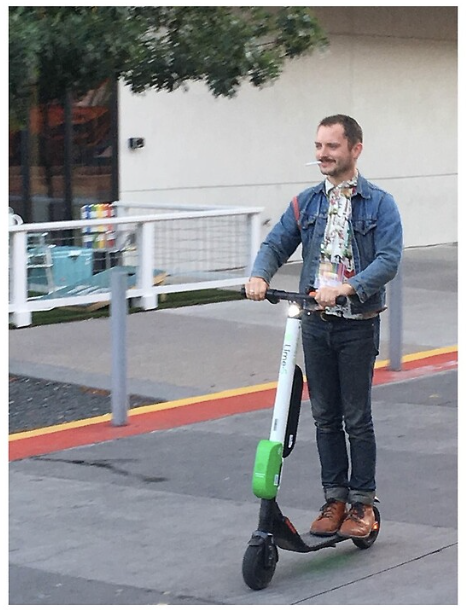
\includegraphics[width=0.5\textwidth]{scooter.png}} % Specify image width and file name
    \caption{Elijah Wood Riding a Lime Scooter}
\end{figure}

\question[3] Elijah Wood, with a mass of $\SI{55}{kg}$, is riding a Lime scooter (mass = $\SI{20}{kg}$) while cruising along at $\SI{5}{m/s}$. Suddenly, Elijah spots the One Ring and jumps \textbf{backwards} off of the scooter at $\SI{2}{m/s}$. How \textbf{fast} will the Lime scooter be going after Elijah jumps off? \\(\emph{Hint:} Use conservation of momentum)


\end{questions}


\end{document}
